\section{Einleitung}
%Security and Privacy in Cloud Computing: Aktuelle Herausforderungen

%Es wird immer wieder fehlende Sicherheit und fehlender Schutz privater Daten in der %Cloud als Hauptargument genannt, warum Firmen die öffentliche Cloud nicht nutzen %wollen. Was wären die aktuelle Herausforderungen und eventeulle Lösungsansätze?

Cloud Computing erlaubt es bei Bedarf über ein Netz auf einen geteilten Pool von konfigurierbaren Ressourcen wie Netzen, Speicher, Anwendungen, Servern und Diensten zuzugreifen. Diese Ressourcen können dabei schnell und mit minimalem Verwaltungsaufwand zur Verfügung gestellt werden \cite{mell2011}. 
Durch diese Eigenschaften des Cloud Computing ergeben sich die folgenden Vorteile \cite{ganesh2014}:
\begin{itemize}
\item 
Erhöhte Flexibilität: Benutzer können einfach und günstig technische Ressourcen erhalten und bei Bedarf wieder freigeben
\item
Reduzierte Kosten: Benutzer müssen sich teuere Ressourcen wie Server nicht mehr kaufen sondern können sich einmieten. Gleichzeitig entfallen deren Wartungskosten. 
\item
Erreichbarkeit: Die erlangten Ressourcen sind im Netz und können von nahezu jedem Ort erreicht werden. Auf die Ressourcen kann zudem mit nahezu jedem Gerät zugegriffen werden das eine Internetverbindung aufbauen kann.
\item
Geteilte Ressourcen: Technische Ressourcen werden von mehreren Nutzern gleichzeitig genutzt, weil niemals alle Nutzer gleichzeitig ihre kompletten Ressourcen ausnutzen können auch kurzzeitige Lastspitzen einzelner Nutzer aufgefangen und gehandhabt werden. Zudem können ungenutzte Ressourcen heruntergefahren werden um die Kosten aller Nutzer zu reduzieren.
\item
Erhöhte Skalierbarkeit: Nutzer können gegen erhöhte Kosten sehr Spontan mehr Ressourcen anfordern um mit einer unerwarteten großen Last nicht überfordert zu sein
\end{itemize}

Neben den Vorteilen gibt es allerdings auch einige Probleme die behandelt werden müssen. So sind Sicherheit und Schutz wichtige Eigenschaften die bei allen kommerziell genutzten Technologien beachtet werden müssen, um Probleme zu vermeiden. Dies gilt auch für alle Ressourcen des Cloud Computing. Gerade bei Anwedungen im öffentlichen Netz gibt es viele potentielle Gefahren, die in der Industrie auch zu finanziellen Verlusten führen können. 
Dabei erstrecken sich die Gefahren von verlorenen Daten, über Betriebsspionage bis hin zu Hardwareschäden. Ein Großteil dieser Gefahren wird in \autoref{sec:fehlender-Schutz} und \autoref{sec:fehlende-Sicherheit} behandelt.
Cloud Computing ist trotz der bekannten Gefahren für viele Firmen ein nützliches Mittel bei der Bewältigung von Aufgaben, sodass die Nutzung von Cloud Computing über die vergangenen Jahre weiter zugenommen hat.
Dass die Industrie dieser Technologie jedoch noch nicht völlig vertraut zeigt sich darin, dass viele Unternehmen viel Geld investieren um die Sicherheit und den Schutz ihrer Cloud Computing Ressourcen zu maximieren. So zeigt sich dieses Verhalten in der 2014 erschienen Umfragestatistik des Markforschungsunternehmens VansonBourne \cite{vansonbourne2014}, aus der hervorgeht dass 58\% aller befragten Unternehmen ihre jährlichen Ausgaben im Bereich der Cloud Sicherheit weiter erhöhen.

Es fehlt an Standards \cite{puthal2015}

\section{Problem: Fehlerhafter Schutz}
\label{sec:fehlender-Schutz}
Fehlender Schutz in Cloud Computing Diensten kann zu Problemen für Cloud Nutzer aber auch für Cloud Anbieter werden. In diesem Kapitel wird auf grundsätzliche Gefahren eingegangen die durch fehlenden Schutz entstehen können.

Im Cloud Computing besteht die Gefahr von Accountdiebstähle oder gekarperte Services. 
Sobald Hacker sich Zugang zu einem Webservice der auf einem Cloud Server läuft verschafft haben, 
können diese eigene Überwachungssoftware auf dem Service installieren 
und so bei gut genutzten Services in kurzer Zeit große Mengen sensibler Informationen von Nutzern des Services erhalten.
Weil die Abhängigkeit von Cloud Computing jährlich zunimmt, 
steigt auch der Schaden solcher Hackerangriffe von Jahr zu Jahr \cite{jabbar2020}. 
 
Durch die hohe Dynamik die durch Cloud Computing geboten wird entstehen weitere neue Angriffsziele. So können zentral verwaltete Mikroservices, die für die Virtualisierung der Infrastruktur einzelner Nutzer eingesetzt werden zum Sicherheitsproblem werden, weil jeder Mikroservice eine andere Systemkonfiguration haben kann \cite{chen2019}. Somit kann jeder Mikroservice andere Sicherheitsrisiken bergen, die ausgenutzt werden können. Ist zudem keine logische Separierung der Ressourcen verschiedener Nutzer gegeben kann durch die Sicherheitslücke eines einzelnen Nutzers auch Schaden an der Cloud Infrasturktur anderer Nutzer verursacht werden \cite{wehrhahn-aklender2019}. In \autoref{fig:sicherheitsproblem} ist ein solcher Angriff dargestellt, bei dem sich durch die virtuelle Maschine eines Nutzers, aufgrund einer fehlende Trennung der virtuellen Ressourcen, Zugang zu einem weiteren Nutzer verschafft werden konnte. 

\begin{figure}[b]
	\centering
	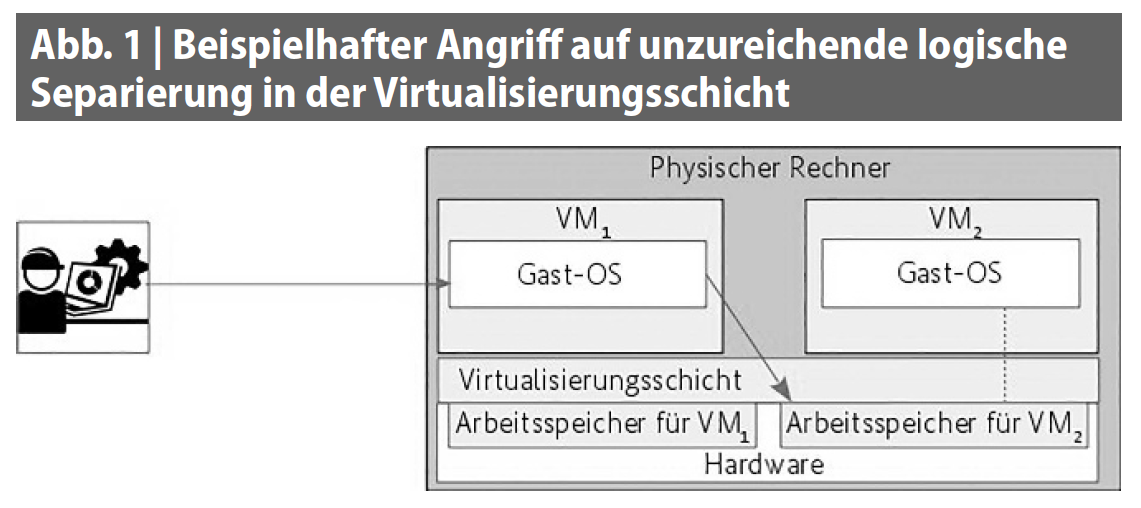
\includegraphics[width=\linewidth]{images/sicherheitsproblem.png}	
	\caption{Gefahr fehlender Trennung virtueller Ressourcen}
	\label{fig:sicherheitsproblem}
\end{figure}

 Kann sich ein Angreifer zugriff auf die Cloud Administration verschaffen hat dieser zudem möglicherweise Zugriff auf die Daten und Services aller Nutzer \cite{wehrhahn-aklender2019}

Weitere Gefahren gehen von cross-site scripting, denial of service Angriffen, 
unsicher programmierten Anwendungen sowie 
data breaches, gehackte interfaces und APIs, defekten Authentifizierungen 
und kompromittierten Berechtigungsnachweise aus. 
Letztere können insbesondere auch zu längeren downtimes und einer reduzierten Verlässlichkeit führen, 
wodurch sich zukünftig die Gefahr von Downtimes erhöhen könnte \cite{jabbar2020}.

\section{Problem: Fehlende Zuverlässigkeit und Verfügbarkeit}
\label{sec:fehlende-Sicherheit}
Durch Ausfälle und um die Hochverfügbarkeit von Cloud Services gewährleisten zu können, 
kommt es Jährlich zu Gewinneinbußen in dreistelliger Millionhöhe \cite{snyder2015 }.
Ausfälle von Cloud Services werden Aufgrund ihres Ausbaus, 
steigender Erfahrung und modernerer Softwarelösungen zwar seltener, 
aber auch heute noch gibt es vereinzelte Ausfälle die Imageschädigend wirken oder zu Einnahmeausfällen geführt haben. 
So gab es zum Beispiel 2017 längere Ausfälle der Cloud Infrasturktur von 
IMB, GitLab, Facebook, Amazon Web Services, Microsoft Azure und Microsoft Office 365. 
Bei den Ausfällen kam es zu Datenverlusten, Zugriffsproblemen von Nutzern auf Accounts, 
Dienste, Projekte und auch kritischen Daten \cite{tsidulko2017}.
%Tsidulko J (2017) The 10 biggest cloud outages of 2017 (So far). 2017; https://www.crn.com/slide-shows/cloud/300089786/the-10-biggest-cloud-outages-of-2017-so-far.htm Accessed 1 Aug 2017


Daten können temporär nicht erreichbar sein oder verloren gehen
Latenzen können gefährliche seiteneffekte haben
Daten können durch fehler öffentlich gemacht werden

\section{Problem: Datensicherheit}
Auch der Wunsch der Benutzer nach Datensicherheit kann eine Herausforderung im Cloud Computing sein. Die Nutzung von Cloud Computing birgt generell datenschutzrechtliche Risiken. 
Persönliche Daten von Nutzern der Clouddienste werden nicht länger lokal gespeichert und gehandhabt sondern von den Cloud Computing Anbietern \cite{selzer2020}. 
Diese Anbieter sind oft internationale Unternehmen, mit Servern die über mehrere Länder verteilt sein können. Je nach Land in dem die Server stehen, gelten eventuell auch andere Richtlinien wie die Sicherheit der Daten gewährleistet werden mussen.




\section{Lösungsansätze}

\subsection{Fehlertollerante Systeme}
Um Datenverluste zu vermeiden und die Verfügbarkeit zu maximieren ist es notwendig fehlertollerantere Systeme aufzubauen. Dazu wurden von Mesbahi \cite{mesbahi2018} aus den Arbeiten von Ganesh et al. \cite{ganesh2014} sowie Jhawar et al. \cite{jhawar2013}die Folgenden Lösungsansätze zusammengetragen.

\begin{itemize}
\item
Präventives Migrieren: Beinhaltet das Speichern der Zustände eines Prozesses, das abschalten von Prozessen, die überführung dieses Zustands zu einem anderen Knoten und die dortige wiederaufnahme des abgeschalteten Prozesses.
Dabei wird ein System eingesetzt, das den Zustand des Prozesses durch Feedbacks regelmäßig überwacht und analysiert. 

\item
Software Verjüngung: Eine Vorbeugende Maßnahme damit sich keine Altlasten in der Laufenden Software ansammeln können. Dabei wird die eingesetzte Software periodisch neu gestartet, um zu vermeiden dass die Software durch verbliebene Altlasten nach und nach Fehler entstehen.
\item
Checkpointing: Durch regelmäßiges Zwischenspeichern des aktuellen Zustands einer Anwendung soll im Falle eines Fehlers die Anwendung wieder in den Zustand zu einem Zeitpunkt gebracht werden können, zu dem die Anwendung Fehlerfrei lief. Dadurch wird vermieden, dass die Anwendung in einem Fehlerfall noch ein mal komplett von Anfang an gestartet werden muss. In einem Fehlerfall wird somit weniger Fortschritt verloren und rechenintensive Schritte müssen eventuell nicht erneut ausgeführt werden.
\item
Redundanz: Durch vervielfachung von Services und Daten kann eine bessere Ausfallsicherheit gewährleistet werden, weil im Falle eines Fehlers auf einer fehlerfreien Kopie des Services weitergearbeitet werden kann. Die Kopien können zudem auf unterschiedliche Systeme aufgeteilt werden, wodurch bei einem Ausfall eines Systems der Service in Form einer identischen Kopie weiterhin zur verfügung steht.
\item
Erneutes Übertragen: Durch erneutes Übertragen eines fehlgeschlagenen Auftrags an den Selben oder einen anderen Host erhält der Service eine weitere Chance den Auftrag korrekt zu verarbeiten. Im Falle eines Netzwerkproblems bei der Übertragung des Auftrags kann so noch ein mal der selbe Auftrag versendet werden, in der Hoffnung, dass es dieses mal zu keinem Netzwerkproblem kommen wird und der Auftrag korrekt ausgeführt wird. EIn Benutzer erfährt durch eine schnelle Ausführung eines erneuten Sendens eventuell gar nicht, dass der ursprüngliche Auftrag fehlgeschlagen ist.

\end{itemize}

\subsection{Datensicherheit} 
\begin{itemize}
\item
Verschlüsseln von physischen Festplatten: Durch das Verschlüsseln von physischen Datenträgern lassen sich die Folgen eines widerrechtlichen Datenabrufs reduzieren, im Falle eines Datenraubs können die geraubten Informationen eventuell gar nicht oder nur mit beträchtlichem Aufwand missbraucht werden \cite{selzer2020}.
\item
Verschlüsseln der Datenübertragung: Durch die Verschlüsselung der Datenübertragung zwischen Cloud Anwendung und Nutzer lässt sich die Gefahr eines Datendiebstahls über eine unsichere Verbindung reduzieren. So können bereits bei der Verschlüsselung physikalischer Datenträger erbeutete Daten nur mit beträchtlichem Aufwand missbraucht werden \cite{selzer2020}.
\item
Pseudonomisierung: Durch die Verschlüsselung von persönlichen Nutzerdaten kann deren  Personenbezug entfernen werden, um einen höheren grad der Anonymisierung bei der Verarbeitung und Speicherung zu erreichen \cite{selzer2020}.
\item
Kontrollen über Zertifikate oder vor Ort: Durch die vermehrte Kontrolle von Zertifikaten von Dritten oder vor Ort bei Anbietern, lässt sich die Korrektheit der Datenverarbeitung bedingt sicherstellen. Nutzer können sich selbst vergewissern, ob ihr Service Datensicherheitskonform arbeitet und dass die sich auf den Servern befindlichen Daten ausreichend gegen äußere Einflüsse geschützt sind \cite{selzer2020}. 
\item 
Datenmetriken: Der Grad des Datenschutzes lässt sich durch Datenmetriken aus Logdaten automatisiert ermitteln. Der Einsatz solcher Metriken erfordert dabei weniger Fachwissen des Prüfers als es bei einer vor Ort Kontrolle benötigt würde, weil das Fachwissen durch die Metriken geliefert wird \cite{selzer2020}. Eine Erweiterung der durch die Metriken erfassten Daten kann dabei zusätzlich mit individuellen Anforderungen ergänzt werden \cite{selzer2020}. Die Datenmetriken lassen sich dabei regelmäßig ausführen, wodurch der Nutzer aktuelle und zeitnahe Informationen über den Zustand der Datensicherheit seines Systems erhält und gegebenenfalls ebenso zeitnah auf Verstöße reagieren kann \cite{selzer2020}.
\item 
Regelmäßige Backups: Durch das regelmäßiges Abspeichern des gesammten Datenbestands lässt sich das Risiko von Datenverlusten reduzieren, indem im Falle eines Hardwareausfalls mithilfe der Backupdaten ein großteil des Datenbestandes wiederhergestellt werden kann.
\end{itemize}


\section{Fazit}
Die von vor Ort Kontrollen durchgeführte Sicherstellung der Datenschutzkonformität hat in ihrer Anwendung nicht die erwünschten Ergebnisse gebracht, weil sich Anbieter auf Kontrollen vorbereitet und Mängel im Vorfeld aus dem Weg geräumt haben \cite{selzer2020}.
Die Qualität von Zertifikate von Drittanbietern lässt sich nicht immer mit Sicherheit bestimmen weil es je nach Land sehr viele unterschiedliche Datenschutz und Datensicherheitszertifizierungen geben kann \cite{selzer2020}.


\cite{inproceedings}

\cite{article}

\cite{patent}

\cite{book}

\cite{electronic}